\documentclass[reprint,english,notitlepage,aps,nobalancelastpage,nofootinbib]{revtex4-1}
\usepackage[utf8]{inputenc}
\usepackage[english]{babel}
\usepackage{physics,amssymb}
\usepackage{graphicx}
\usepackage{xcolor}
\usepackage{hyperref}
\usepackage{tikz}
\usepackage{listings}
\usepackage{subfigure}
\usepackage{amsmath,mathtools}
\usepackage{amsbsy}
\usepackage{enumitem}
\usepackage{bbold}

\graphicspath{{../plots/}}

\hypersetup{
    colorlinks,
    linkcolor={red!50!black},
    citecolor={blue!50!black},
    urlcolor={blue!80!black}}

\lstset{
	inputpath=,
	backgroundcolor=\color{white!88!black},
	basicstyle={\ttfamily\scriptsize},
	commentstyle=\color{magenta},
	language=Python,
	morekeywords={True,False},
	tabsize=4,
	stringstyle=\color{green!55!black},
	frame=single,
	keywordstyle=\color{blue},
	showstringspaces=false,
	columns=fullflexible,
	keepspaces=true}


\newcommand{\closed}[1]{\left(#1\right)}
\newcommand{\bracket}[1]{\left[#1\right]}

\newcommand{\tmdv}[4]{\closed{\pdv{#1}{#2}}_{#3,#4}}
\newcommand{\jacobian}[2]{\pdv{(#1)}{(#2)}}
\renewcommand{\d}{\mathrm{d}}
\newcommand{\sumstate}{\sum_{\{\sigma_j\}}}
\newcommand{\prodstate}{\prod_{i=0}^{L-1}}
\newcommand{\ebj}{e^{\beta J}}
\newcommand{\T}[1]{T_{\sigma_{#1},\sigma_{#1 + 1}}}
\renewcommand{\l}{\lambda}
\newcommand{\mj}{m_j}

\begin{document}
\begin{center}
\title{\Huge FYS4130 - Oblig 2}
\author{\large Vetle A. Vikenes}
\date{\today}
\noaffiliation


\maketitle
\end{center}
\onecolumngrid

All code used in this oblig can be found on my Github: \url{https://github.com/Vikenes/FYS4130}
\\
\section*{\large Task 1 - Transfer Matrices}

\subsection*{a) Partition function and average internal energy}

We consider a 1D spin chain of length $L$ with periodic boundary conditions. The Hamiltonian of the system given as  
\begin{align} \label{eq:Hamiltonian}
	H &= -J \sum_{i=0}^{L-1} \delta_{\sigma_i,\sigma_{i+1}},
\end{align}

where $\sigma_i=\{0,\,1,\,2\}$ denotes the spin at site $i$ and $J>0$.    

The order parameter, $m$, and local magnetization, $m_j$, is given by
\begin{align}
	m &\equiv \frac{1}{N} \sum_{j=0}^{N-1} m_j \label{eq:order parameter}  \\ 
	\text{where}\quad m_j &\equiv e^{i(2\pi/3)\sigma_j} \label{eq:magnetization}
\end{align}

To calculate the partition function, we begin by inserting the expression for the Hamiltonian and write the sum in the exponent in terms of products. 
\begin{align*}
	Z &= \sum_{\{\sigma_j\}} e^{-\beta H} = \sumstate e^{\beta J \sum_{i=0}^{L-1} \delta_{\sigma_i,\sigma_{i+1}}} = \sumstate \prod_{i=0}^{L-1} e^{\beta J \delta_{\sigma_i,\sigma_{i+1}}}
\end{align*}

The exponential can be written in terms of transfer matrices representing the different values of the exponential for different spin states. Letting $\sigma_i$ and $\sigma_{i+1}$ govern the row and column, respectively, the transfer matrix becomes 

\begin{align*}
	T_{\sigma_i,\sigma_{i+1}} &= 
	\begin{pmatrix}
		e^{\beta J} & 1 & 1 \\
		1 & \ebj & 1 \\
		1 & 1 & \ebj
	\end{pmatrix}.
\end{align*}

The transfer matrix will thus look identical for different values of $\sigma_i$, so taking the product between different ones, results in a transfer matrix raised to a certain power.  

\begin{align*}
	Z &= \sumstate \prodstate \T{j} = \sumstate T_{\sigma_0,\sigma_1} T_{\sigma_1,\sigma_2}\cdots T_{\sigma_{L-1},\sigma_0} 
\end{align*}
where we invoked the periodicity, $\sigma_L=\sigma_0$, in the last line. This means that we're summing over repeated indices, and the sum can be carried out by taking the trace of the resulting matrix products. To calculate the product of the matrices, we start by diagonalizing it

\begin{align*}
	\begin{pmatrix*}[r]
		-1 & -1 & 0 \\ 
		2 & 1 & 1 \\ 
		2 & 1 & 0 
	\end{pmatrix*}
\end{align*}

\begin{align*}
	T &= PDP^{-1}, \:\mathrm{where}\: \\ 
	P &= 
	\begin{pmatrix*}[r]
		-1 & -1 & 1 \\ 
		0  & 1  & 1 \\ 
		1  & 0  & 1 
	\end{pmatrix*} ,\quad 
	P^{-1} = \frac{1}{3} \begin{pmatrix*}[r]
		-1 & -1 & 2 \\ 
		-1 & 2  & -1 \\ 
		1  & 1  & 1
	\end{pmatrix*}
	,\quad D = \begin{pmatrix*}[r]
		\lambda_1 & 0 & 0 \\ 
		0 & \lambda_2 & 0 \\
		0 & 0 & \lambda_3 
	\end{pmatrix*}
\end{align*}

The eigenvalues of $T$ are 
\begin{align*}
	\lambda_1 &= \ebj-1 \\ 
	\lambda_2 &= \ebj-1 \\ 
	\lambda_3 &= \ebj+2
\end{align*}


\begin{align*}
	Z &= \Tr(SDS^{-1}SDS^{-1}\cdots DS^{-1})=Tr(D^L)=2\lambda_1^L + \lambda_3^L \\ 
	&= 2(\ebj-1)^L + (\ebj+2)^L
\end{align*}

\begin{align*}
	U &= \pdv{(\beta F)}{\beta}
\end{align*}

\begin{align*}
	\beta F = -\ln Z = -\ln(2)-L\ln(\ebj-1)-L\ln(\ebj+2)
\end{align*}

\begin{align*}
	U = -L \frac{J\ebj}{\ebj-1} - L \frac{J\ebj}{\ebj+2}
\end{align*}

For an approximate expression of $U$ we can rewrite the partition function in a way that allows us to neglect a term. 
\begin{align*}
	Z = 2\l_1^L + \l_3^L = \l_3^L\bracket{2\closed{\frac{\l_1}{\l_3}}^L+1}
\end{align*} 
For large $L$ there are two limiting cases. If $\beta$ is very large $\l_1/\l_3\approx1$ so $Z\approx 3\l_3^L$. If, on the other hand, $\beta$ is small we get $Z\approx \l_3^L$, as the fraction goes to zero when $L$ becomes large. Since we have to differentiate the logarithm of $Z$ with respect to $\beta$ to obtain the approximate expression for $U$, the constant in front of $\l_3^L$ is irrelevant. An approximate expression for $U$ is thus 
\begin{align*}
	U&=-\pdv{\beta}\ln Z \approx -\pdv{\beta} L \ln \l_3 = -L \pdv{\beta}\ln (\ebj+2) \\ 
	&= -\frac{LJ}{1+2 e^{-\beta J}} 
\end{align*}

For $T\to0$ the approximate expression for $U$ becomes 
\begin{align*}
	\lim_{\beta\to\infty} U = -LJ
\end{align*}
and for $T\to\infty$ we get 
\begin{align*}
	\lim_{\beta\to0} U = -\frac{LJ}{1+2}=-\frac{LJ}{3}
\end{align*}

In the low temperature limit we get the minimum energy of our model, where all the spins are aligned. In the high temperature limit, we have disordered spin states. Since $\sigma_j$ can take three possible values, the probability of neighbouring spins being aligned is $1/3$, and we thus get one third of the total available energy.  


\subsection*{b) - Average magnetization}

\begin{align*}
	\expval{m} = \frac{1}{N} \sum_{i=0}^{N-1}\expval{m_j}
\end{align*}


\begin{align*}
	\expval{m_j} &= \frac{1}{Z} \sumstate \mj e^{-\beta H} = \frac{1}{Z} \sumstate e^{i(2\pi/3)\sigma_j} \prodstate e^{\beta J \delta_{\sigma_i,\sigma_{i+1}}} \\ 
	&= \frac{1}{Z} \sum_{\sigma_0} \sum_{\sigma_j} T_{\sigma_0,\sigma_j}^j e^{i(2\pi/3)\sigma_j} T_{\sigma_j,\sigma_0}^{L-j}
\end{align*}
To carry out the sum, we now use that we sum over repeated indices and we thus have to compute the trace of the resulting matrix. It can be shown that the matrix product $PDP^{-1}$ will have the same entries on its diagonal, due to the fact that $\l_1=\l_2$. This implies that the product of the two matrices in our equation for $\expval{\mj}$ will also have the same entries on its diagonal, so the expression becomes
\begin{align*}
	\expval{\mj} &= \frac{1}{Z} \closed{T_{0,0}^j\,T_{0,0}^{L-j} + e^{i2\pi/3} \,T_{1,1}^j\,T_{1,1}^{L-j} + e^{-i2\pi/3}\,T_{2,2}^j\,T_{2,2}^{L-j}} \\ 
	&= \frac{1}{Z} \closed{1 + e^{i2\pi/3} + e^{-i2\pi/3}} 3\,T_{0,0}^{j} \, T_{0,0}^{L-j} \\ 
	&= 0
\end{align*}  
since the sum of spins equals $0$. Thus, we have $\expval{\mj}=0$, which then implies

\begin{align*}
	\expval{m} = 0,
\end{align*}
which is what we wanted to show.

\subsection*{c) - Correlation function}
The correlation function is defined as 
\begin{align} \label{eq:corr_func}
	C(r) &\equiv \expval{m_0^* m_r} - \expval{m_0^*}\expval{m_r}.
\end{align}
Having already found that $\expval{\mj}=0$, the last term in equation \eqref{eq:corr_func} vanishes, and we're left with the quantity $\expval{m_0^* m_r}$, which we can write in terms of exponentials as 

\begin{align*}
	\expval{m_0^* m_r} &= \expval{e^{i(2\pi/3)(\sigma_r - \sigma_0)}}.
\end{align*}

We follow the same procedure as before, writing out all sums except for the ones over $\sigma_0$ and $\sigma_r$ this time. 

\begin{align*}
	\expval{m_0^* m_r} &= \frac{1}{Z} \sumstate m_0^* m_r \, \prodstate \T{i} = \frac{1}{Z} \sum_{\sigma_0} \sum_{\sigma_r} e^{i\frac{2\pi}{3}(\sigma_r-\sigma_0)} T_{\sigma_0,\sigma_r}^{r} \, T_{\sigma_r,\sigma_0}^{L-r} 
\end{align*}

Now, the exponential term will contribute differently depending on the relative difference between the two spins. Using the diagonalization $T=PDP^{-1}$ we write the general expression for $T_{i,j}^k$ by performing the matrix multiplications. The resulting matrix will have identical terms on the diagonal, as well as identical terms on the off-diagnoal. These terms are given in equation \eqref{eq:T_power}  

\begin{align} \label{eq:T_power}
	T_{i,j}^k = \frac{1}{3}\begin{cases}
		2(\ebj-1)^k + (\ebj+2)^k \quad &\mathrm{for}\; i=j \\ 
		-(\ebj-1)^k + (\ebj+2)^k \quad &\mathrm{for}\; i\neq j
	\end{cases}
\end{align}

When we sum over the two spins, we will get three identical contributions from the diagonal, since the exponential term is $1$ in this case. Since the off-diagonal elements are identical, there will be three identical terms with a factor $e^{i2\pi/3}$ as well as three identical terms with a factor $e^{-i2\pi/3}$. To simplify the writing, we express these three different contributions with the matrix elements $T_{0,0},\,T_{0,1}$ and $T_{1,0}$, corresponding to the common factors $1,\,e^{i2\pi/3}$ and $e^{-i2\pi/3}$, respectively. Omitting the explicit computation of the products, we simply insert the results.  

\begin{align*}
	\expval{m_0^* m_r} = \frac{1}{Z} \Big[ &3\, T_{0,0}^r T_{0,0}^{L-r} + 3e^{i2\pi/3}\, T_{0,1}^r T_{1,0}^{L-r} + 3e^{-i2\pi/3}\, T_{1,0}^r T_{0,1}^{L-r} \Big] \\ 
	= \frac{1}{Z} \frac{1}{3} \Bigg[ &4(\ebj-1)^L + 2(\ebj-1)^r (\ebj+2)^{L-r} + 2 (\ebj+2)^r (\ebj-1)^{L-r} + (\ebj+2)^L \\
	& + e^{i2\pi/3}\bracket{ (\ebj-1)^L + (\ebj+2)^L - (\ebj-1)^r (\ebj+2)^{L-r} - (\ebj+2)^r (\ebj-1)^{L-r} } \\
	& + e^{-i2\pi/3} \bracket{(\ebj-1)^L + (\ebj+2)^L - (\ebj-1)^r (\ebj+2)^{L-r} - (\ebj+2)^r (\ebj-1)^{L-r}} \Bigg] \\ 
	= \frac{1}{Z}\frac{1}{3} \Bigg[ & 4(\ebj-1)^L + (\ebj+2)^L + 2(\ebj-1)^r (\ebj+2)^{L-r} + 2 (\ebj+2)^r (\ebj-1)^{L-r} \\
	& - (\ebj-1)^L - (\ebj+2)^L + (\ebj-1)^r (\ebj+2)^{L-r} + (\ebj+2)^r (\ebj-1)^{L-r} \Bigg] \\ 
	= \frac{1}{Z} \frac{1}{3} \Bigg[ & 3(\ebj-1)^L + 3 (\ebj-1)^r (\ebj+2)^{L-r} + 3 (\ebj+2)^r (\ebj-1)^{L-r} \Bigg],
\end{align*}
where we used that $e^{i2\pi/3} + e^{-i2\pi/3}=-1$. Canceling the common factors of $3$ and writing out the partition function, our final expression for the correlatino function becomes 

\begin{align} \label{eq:corr_func_result}
	C(r) &= \frac{(\ebj-1)^L + (\ebj-1)^r (\ebj+2)^{L-r} + (\ebj-1)^{L-r} (\ebj+2)^r}{2(\ebj-1)^L + (\ebj+2)^L}
\end{align}

Using WolframAlpha we find the expression for $C(r)$ in the limiting case $L\to\infty$
\begin{align*}
	\lim_{L\to\infty} C(r) = \closed{\frac{\ebj-1}{\ebj+2}}^r = \closed{\frac{\l_1}{\l_3}}^r
\end{align*}
For $T=0$, we use WolframAlpha ones again to find the limit as $\beta\to\infty$ and get 
\begin{align*}
	\lim_{T\to0} C(r) = 1.
\end{align*}


\section*{\large Task 2 - Monte Carlo Simulations}


\begin{figure}[h!]
	\centering
	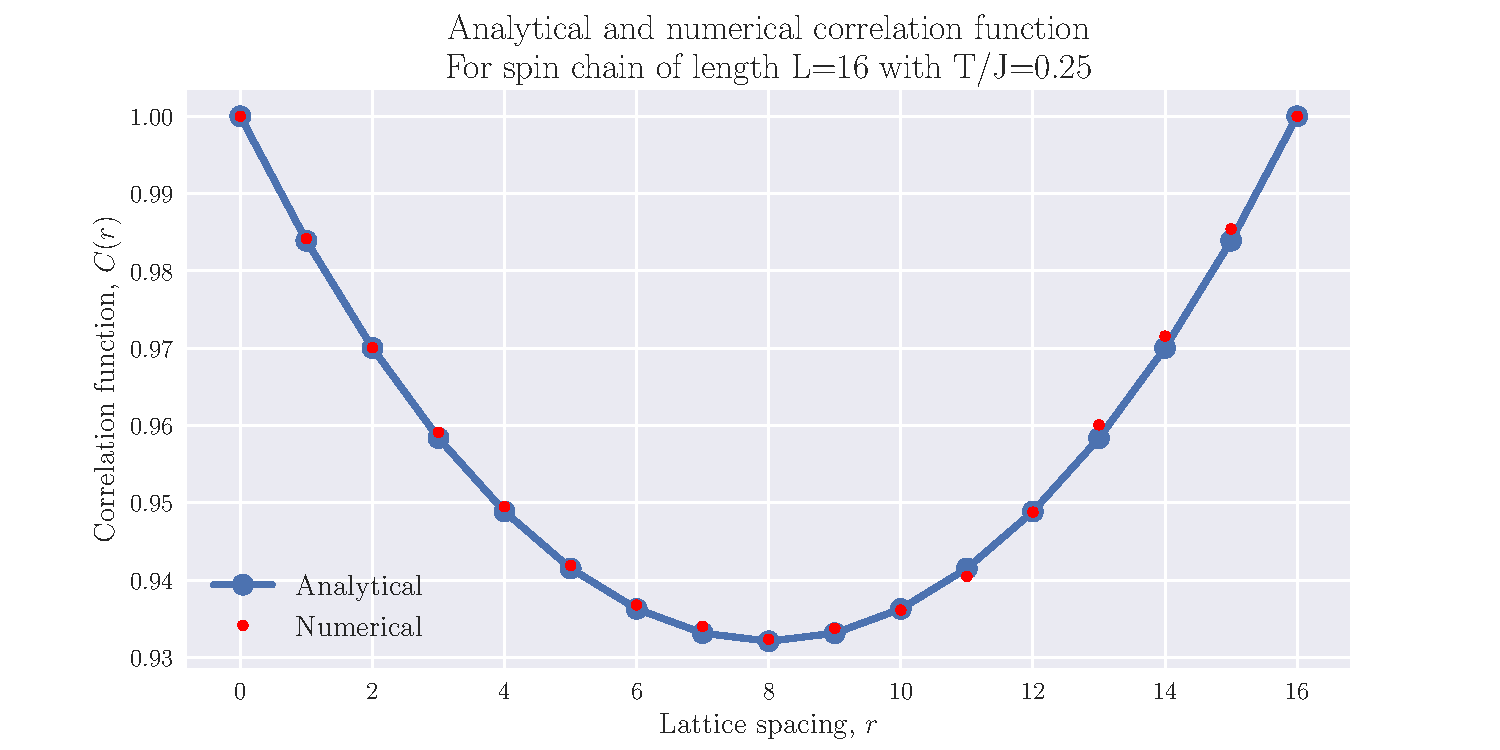
\includegraphics[width=0.7\linewidth]{correlation1D_025.pdf}
	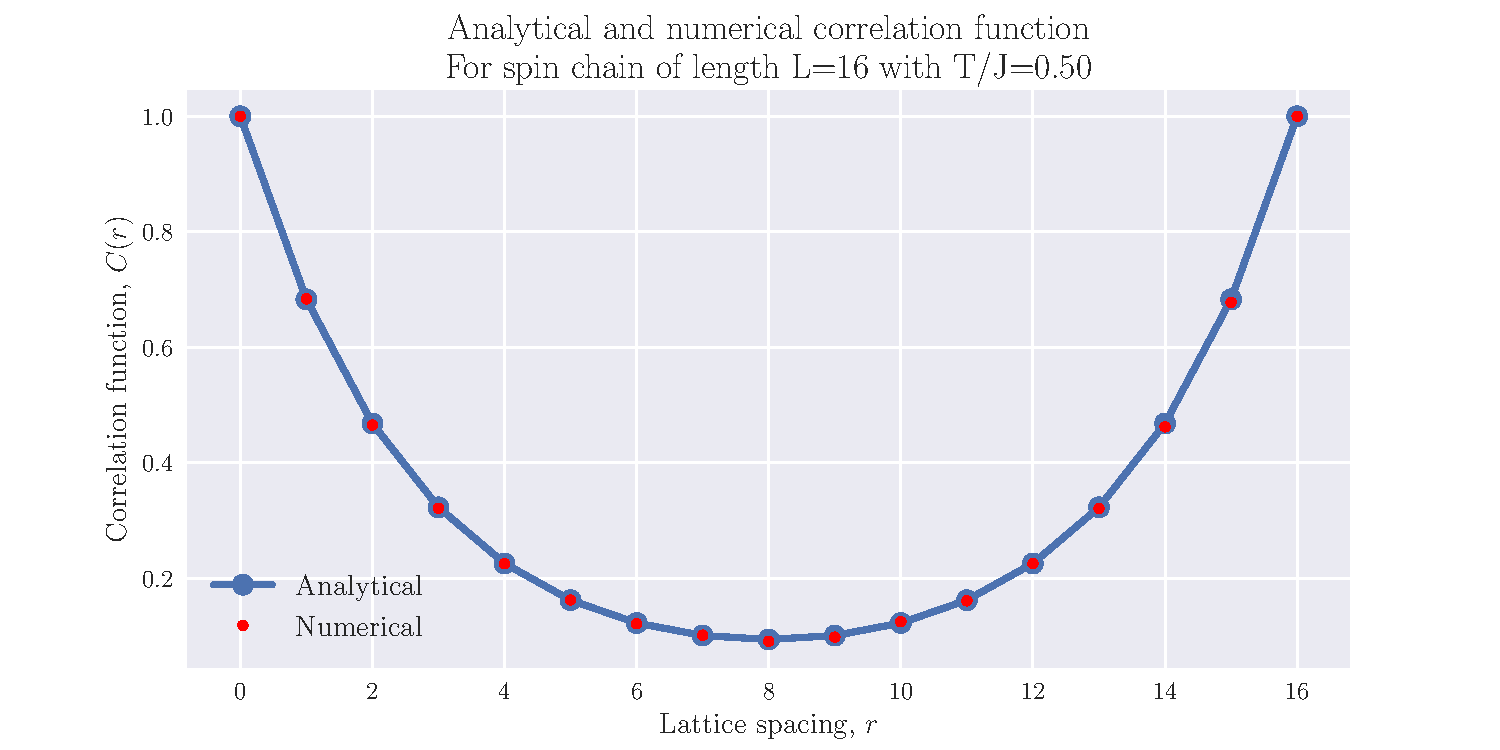
\includegraphics[width=0.7\linewidth]{correlation1D_05.pdf}
	\caption{Correlation}
	\label{fig:correlation}
\end{figure}


\end{document}
